\section{Nguyên lý hoạt động}
\subsection{Chuyển chế độ}
\begin{figure}[H]
    \centering
    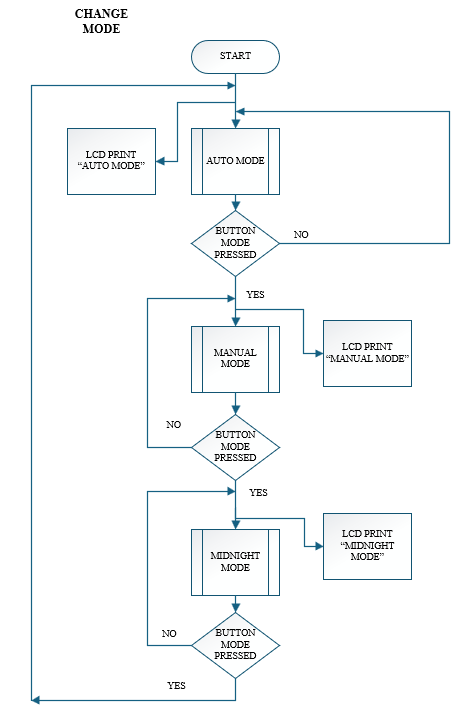
\includegraphics[width=0.8\textwidth]{pictures/modes.png}
    \caption{Lưu đồ chuyển chế độ}
\end{figure}
\cleardoublepage
Lưu đồ chuyển chế độ mô tả trình tự xử lý nút nhấn để thay đổi chế độ hoạt động của hệ thống đèn giao thông. Sau khi khởi động, hệ thống bắt đầu ở chế độ AUTO MODE, đồng thời hiển thị dòng chữ “AUTO MODE” trên LCD. Trong mỗi chế độ, hệ thống liên tục kiểm tra xem nút MODE có được nhấn hay không:
\begin{itemize}
    \item Chế độ mặc định là chế độ tự động (AUTO MODE).
    \item Nếu nút nhấn chuyển trạng thái không được nhấn, hệ thống tiếp tục duy trì chế độ hiện tại.
    \item Nếu nút nhấn chuyển trạng thái được nhấn, hệ thống sẽ chuyển sang chế độ tiếp theo trong danh sách chế độ hoạt động. 
    \item Sau mỗi lần chuyển chế độ LCD sẽ cập nhật lại dòng chữ hiển thị chế độ tương ứng.
\end{itemize}
\subsection{Chế độ tự động}
\begin{figure}[H]
    \centering
    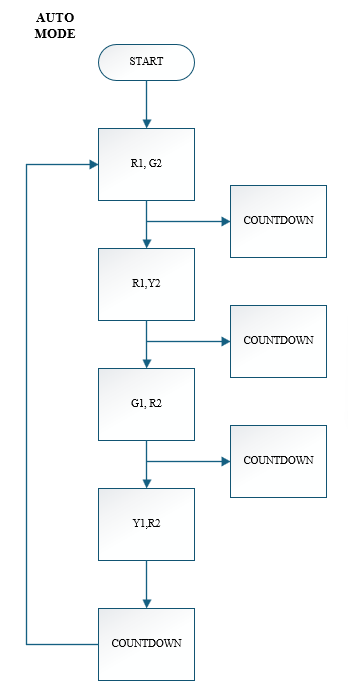
\includegraphics[width=0.45\textwidth]{pictures/auto.png}
    \caption{Lưu đồ chế độ tự động}
\end{figure}
\cleardoublepage
Chế độ tự động mô phỏng hoạt động thực tế của hệ thống đèn giao thông. Lưu đồ mô tả thứ tự bật/tắt đèn theo chu kỳ, kết hợp với bộ đếm thời gian:
\begin{enumerate}
    \item Bật \textbf{R1, G2} $\rightarrow$ đếm ngược
    \item Bật \textbf{R1, Y2} $\rightarrow$ đếm ngược
    \item Bật \textbf{G1, R2} $\rightarrow$ đếm ngược
    \item Bật \textbf{Y1, R2} $\rightarrow$ đếm ngược
\end{enumerate}


Sau bước cuối, hệ thống quay lại bước đầu tiên để lặp lại chu kỳ. Đây là chế độ giao thông tiêu chuẩn cho hai hướng đối diện.
\subsection{Chế độ thủ công}
\begin{figure}[H]
    \centering
    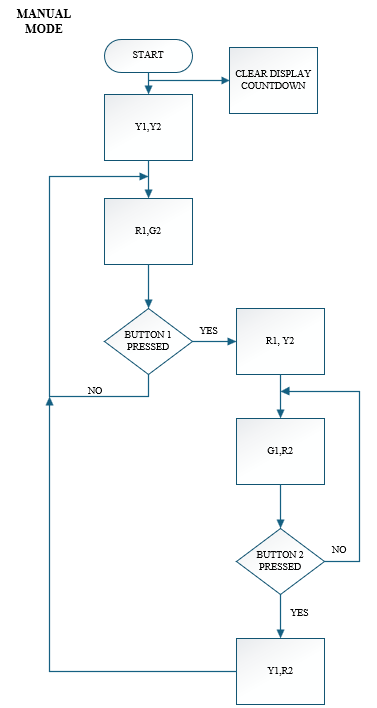
\includegraphics[width=0.7\textwidth]{pictures/manual.png}
    \caption{Lưu đồ chế độ thủ công}
\end{figure}
\cleardoublepage
Trong chế độ này, người dùng chủ động điều khiển các giai đoạn đèn giao thông thông qua nút nhấn.

Trình tự hoạt động như sau:

\begin{enumerate}
  \item Bật \textbf{R1, G2}
  \item Chờ nhấn \textbf{BUTTON 1}. Nếu không nhấn, giữ nguyên trạng thái.
  \item Nếu BUTTON 1 được nhấn, chuyển sang \textbf{G1, R2}
  \item Chờ nhấn \textbf{BUTTON 2}. Nếu không nhấn, giữ nguyên trạng thái.
  \item Nếu BUTTON 2 được nhấn, chuyển sang \textbf{R1, G2}, sau đó quay lại bước đầu tiên.
\end{enumerate}

Chế độ này thích hợp để điều phối giao thông theo yêu cầu trong các tình huống đặc biệt.

\subsection{Chế độ ban đêm}
\begin{figure}[H]
    \centering
    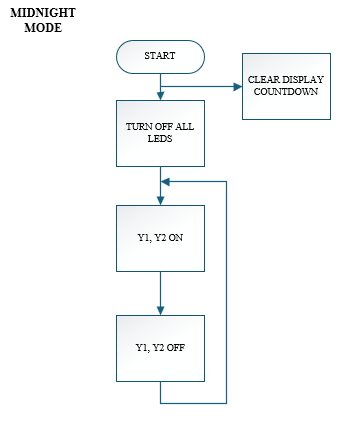
\includegraphics[width=0.7\textwidth]{pictures/night.png}
    \caption{Lưu đồ chế độ ban đêm}
\end{figure}
\cleardoublepage
Chế độ ban đêm giúp tiết kiệm điện năng và tăng cảnh báo cho các phương tiện giao thông khi lưu lượng thấp. Trình tự hoạt động:

\begin{enumerate}
  \item Khởi động và xóa màn hình LCD
  \item Tắt toàn bộ đèn (\textbf{OFF ALL LEDs})
  \item Bật \textbf{Y1, Y2} $\rightarrow$ đèn vàng hai hướng sáng
  \item Tắt \textbf{Y1, Y2}
  \item Quay lại bước bật Y1, Y2 để tạo hiệu ứng nhấp nháy liên tục
\end{enumerate}

Chế độ này đảm bảo cảnh báo tối thiểu nhưng không gây cản trở phương tiện trong đêm khuya.